\chapter{Model Stability} \label{stability}

When we start to care about modelling multiple nanowires and including more complicated dynamics
(such as thermal devices, hTrons, or multiport nanowires, nTrons), the stability of the underlying
base model is crucial. The nanowire model is the basis for all these models and is unreliable leading
to switching behavior due to its non-linearities constantly. The SPICE environment wasn't built to
handle harsh non-linearities such as the state non-linearity and therefore requires a careful
analysis of how submodels interact together to guarantee the correctness and stability of the model.
We introduce a simple enumerative method that can be used to debug non-linear (and linear) circuits
and compare their stability. We then use this method to improve the stability of the nanowire model
by changing the hotspot integrator.

\section{Integration in SPICE}

SPICE implementations in general rely on second-order integration, namely trapezoidal and Gear integration. LTspice allows the user to pick between 4 options: trapezoidal,
Gear, (1st Order) Backward Euler and a proprietary modified trapezoidal method. In general,
Backwards is the most stable and least accurate, followed by Gear integration 
\cite{ltspice-diff-post, spice-book}.

Trapezoidal integration is generally faster and more accurate than Gear but introduces a ringing
numerical artifact that occurs at adjacent timesteps on stiff systems. Ringing is dampened by the Gear
method causing this numerical artifact to be mostly eliminated. The Gear method achieves that by
dampening most ringing as shown in figure \ref{fig:trapz_vs_gear}. The setup in figure \ref{fig:trapz_vs_gear} uses an nanowire-capacitor oscillator working in the linear regime starting
with an initial amount of energy.
We typically care about oscillatory behavior in nanowires that can be filtered by the Gear
method (especially in the timeframe shown)
and as a result, we choose to use the trapezoidal method. LTspice's 
default integration method is a proprietary modified version of trapezoidal integration 
that cancels out the trapezoidal ringing introduced by the regular implementation without
numerical dampening \cite{ltspice-diff-post}. 

\begin{figure}
    \centering
    \subfigure[]{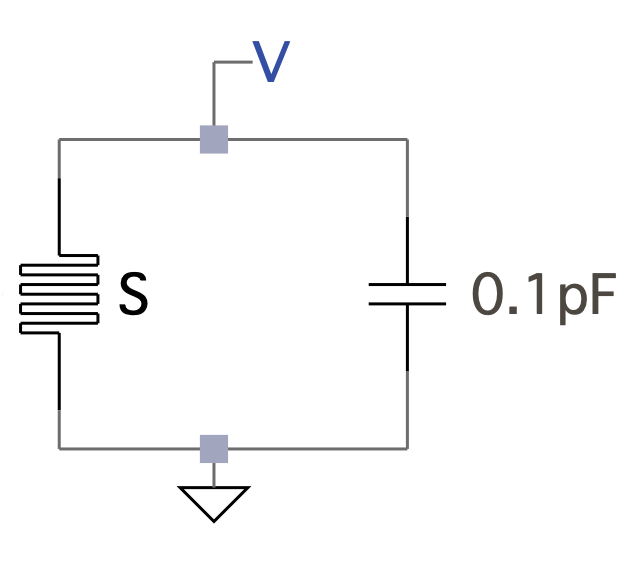
\includegraphics[width=0.3\textwidth]{figs/method_vs_Circ.png} \label{fig:tank_circ}}
    \subfigure[]{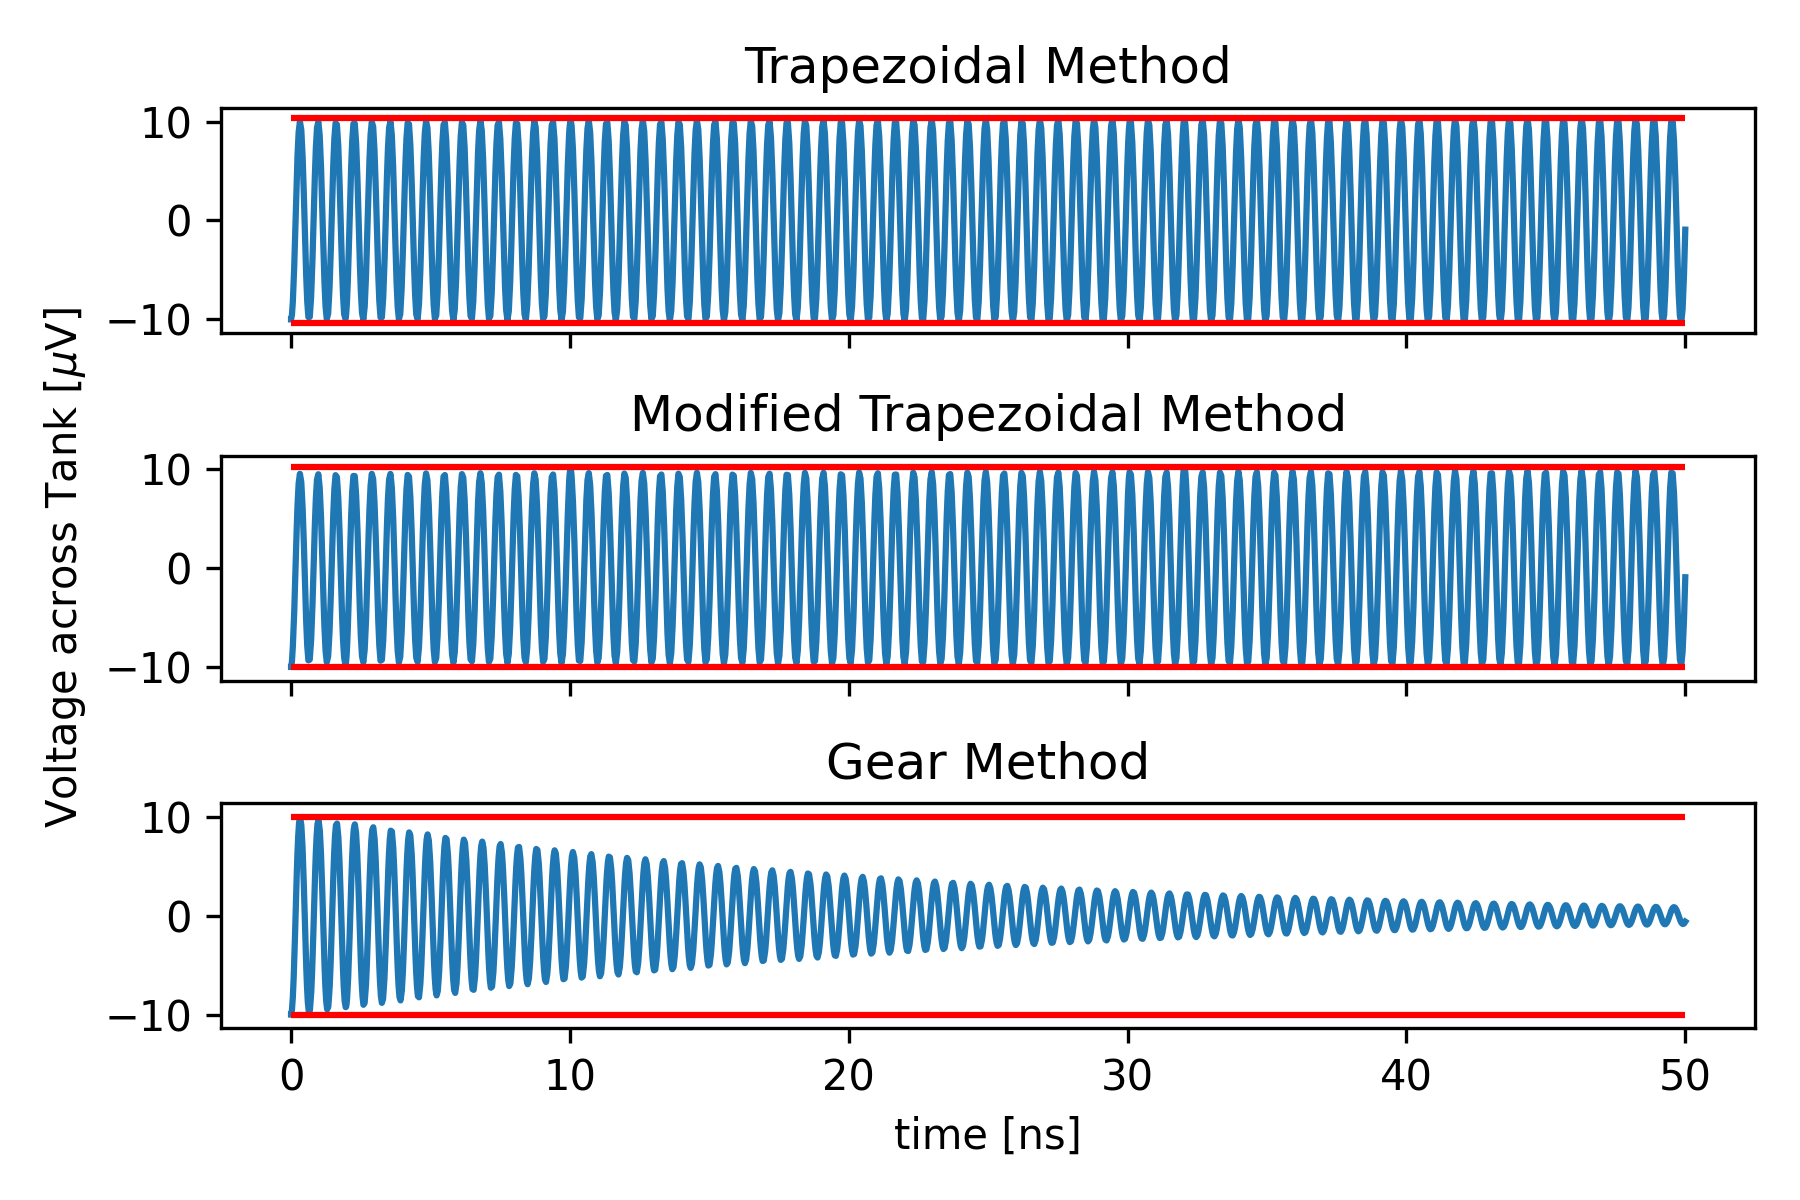
\includegraphics[width=0.67\textwidth]{figs/method_vs.png}}
    \caption{Comparison of the 3 different second-order integration methods
    LTspice is equipped to use. (a) An LC resonator that uses a non-linear inductor
    (nanowire) in parallel with a capacitor. The initial condition for node \cf{V} is set
    to $100\mu$V.
    (b) The voltage as a function of time
    computed using the 3 different integration methods. Gear method causes significant
    signal decay when there shouldn't be decay at timescales we typically care about 
    in nanowires. The modified trapezoidal method
    has less consistent magnitudes of the output sine wave.}
    \label{fig:trapz_vs_gear}
\end{figure}

\section{Stability in Transient Simulations}

Stability of a finite element method is intimately related to the consistency and convergence of
the method through the Dahlquist Equivalence Theorem \cite{DAHLQUIST}. 
One result of this for non-linear systems,
such as the nanowire model, is their solution should be smooth as you decrease the timestep.
As in, there must exist a timestep $\Delta t$ for which all timesteps $< \Delta t$ the method
gives a result bounded around that of using the timestep $\Delta t$. Transient simulations, which are a 
type of continuation method parametrized with time, often use straightforward convergence correction. 
In this method, the timestep for continuous signals is decreased until convergence is achieved, 
which is guaranteed to occur for continuous signals \cite{spice-book}.

One way of visualizing solving a continuous system using a finite element method is by
represent timestep corrections
as projections. For instance, solving for the final state $u(T)$ for a circuit $C$ at a time $T$ 
transforms $u(0)\xrightarrow[]{} u(T)$ smoothly when continuous. However, when a finite method is used
with coarse discretizations, the method steps around this continuous evolution. Overshoots due to the
coarseness could exist outside the state-space and the solution trajectory but are corrected for
as illustrated in figure \ref{fig:statespaceevolution}. 
These corrections (decreasing the timestep and adding gmin capacitances) can be thought of as projections
back into the subspace of possible solutions. The subspace of possible solutions is
a lightcone around the current state where the size of the lightcone is constrained
by the circuit topology and simulation parameters such as \cf{reltol}. The lightcone
of a state is the set of states you can reach from that state in one timstep. The
lightcone of a target state is the set of states that can reach it in one timestep.

In a non-linear system, these projections can lead to integrating errors. Consider the
state non-linearity for instance, if a projection happens to enter that regime at any
point in the simulation accidentally, it would cause a misfire. Now consider the coupling
of this to the continuous non-linearity which amplifies values. This amplification can
make it easier to reach the state non-linearity lightcone and accidentally trigger
the hotspot integrator.

\begin{figure}
    \centering
    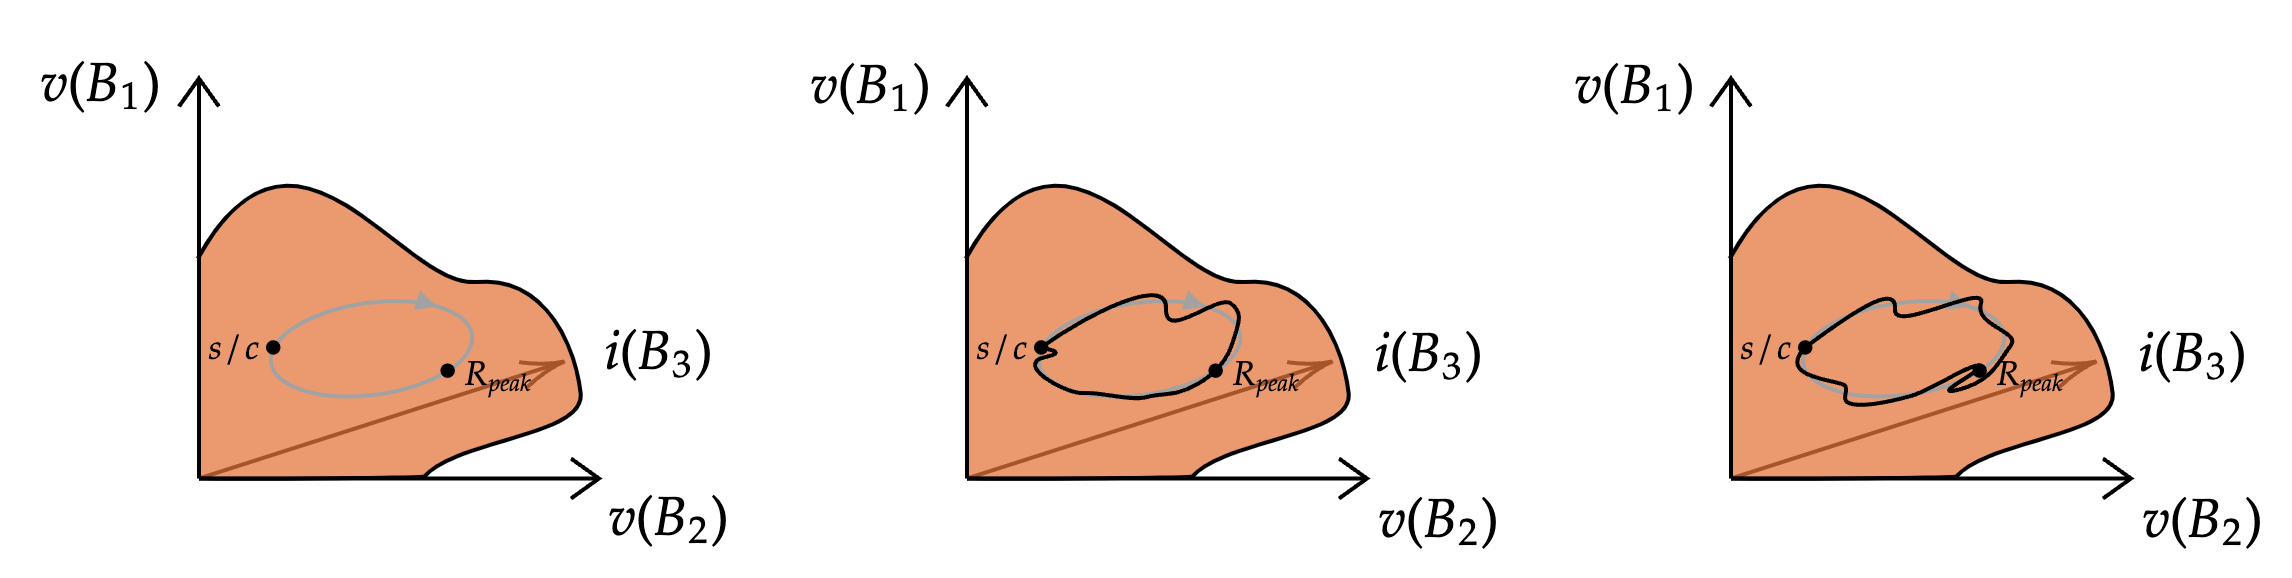
\includegraphics[width=0.9\textwidth]{figs/statespaceevolution.png}
    \caption{A notional diagram of the evolution of a circuit simulation for a nanowire.
    The orange space represents all the states (combinations of node voltages and currents) 
    that the circuit can be in. The experimentally-observed continuous dynamics of the nanowire follow
    the gray line's evolution between two points, the superconducting (s/c) state and the maximum resistance
    state ($R_{peak}$). The system in the first plot encodes multiple simple configurations of superconducting nanowires, such as SNSPDs and relaxation oscillations, with the three axes being the behavioral sources in the nanowire model. A nanowire in the superconducting state starts at the (s/c) node. When a photon is incident, it begins to evolve around the path crossing through $R_{peac}$ and
    returning to the (s/c) node. The second diagram shows a finite approximation of this path that a solver
    might take, meanwhile producing the correct number of state transitions. The third diagram shows
    how a projection caused by a finite method could cause the wire to trigger twice. The finite method
    overshoots $R_{peak}$, corrects to before it, and crosses it again (causing two SNSPD spikes).}
    \label{fig:statespaceevolution}
\end{figure}

\subsection{Stability of the Nanowire Model} 

Boolean state non-linearities are integral to optimizing and training Neural Networks, and as a 
result are a well studied concept. A common way of solving this issue is smoothening out the 
change by modeling the boolean state as a continuous state transition with a smooth interpolating
function, such as a sigmoid function. In nanowires, we particularly care about smoothness of state
transition over time while the transition dependence is on current (which is also a function of time).
Macroscopically, this state transition involves a chain reaction and can be modelled as a smooth
ramp up (the hotspot thermal growth is a smooth change). This is how the hotspot integrator in the 
existing nanowire model handles the non-linear transition into the resistive state.

The nanowire model is unstable and inconsistent over both Boolean and continuous non-linearities (discussed in section \ref{nonlinearity}) in a disguised 
fashion. While this can be improved by tweaking the relative tolerance (\cf{reltol}) 
of the simulation, improving the model's stability is essential to scaling devices and integration 
with other circuits.
One big issue with the instability is the behavior of the model is not out of question, in that,
even though the solution is incorrect, it looks plausible. For instance, you might see extra counts
when you aren't supposed to see them when you include tapers (due to the modified time-stepping behavior
for circuits when tapers are included, discussed in \ref{tapers_section}). Other instability effects
include things like pre- and post-firing of the nanowire, which can be hard to discern from reflections
occurring in the circuit that might actually cause the wire to re-fire.

This instability over the non-linearity is amplified due to the time-stepping. An approximate 
solution to a non-linear system has a response dependent on the magnitude at the previous timestep. 
As a result,
near portions of the transfer functions that can't be approximated as linear, a projection
onto an acceptible relative tolerance value at timestep $n$ does not correspond to an
acceptable relative tolerance at a timestep $n+1$ due to the magnitude dependence.
This forward propagation of error explains false switching events at timesteps that
are too close together caused by a time-coupled element (more on that in \ref{malicious_circuits}).
We see this in effect in figure \ref{fig:sweepbias} with multiple false switching events.

\subsection{Relative Tolerance for the Nanowire Model} \label{reltol}

\begin{figure}
    \centering
    % \subfigure[]{
    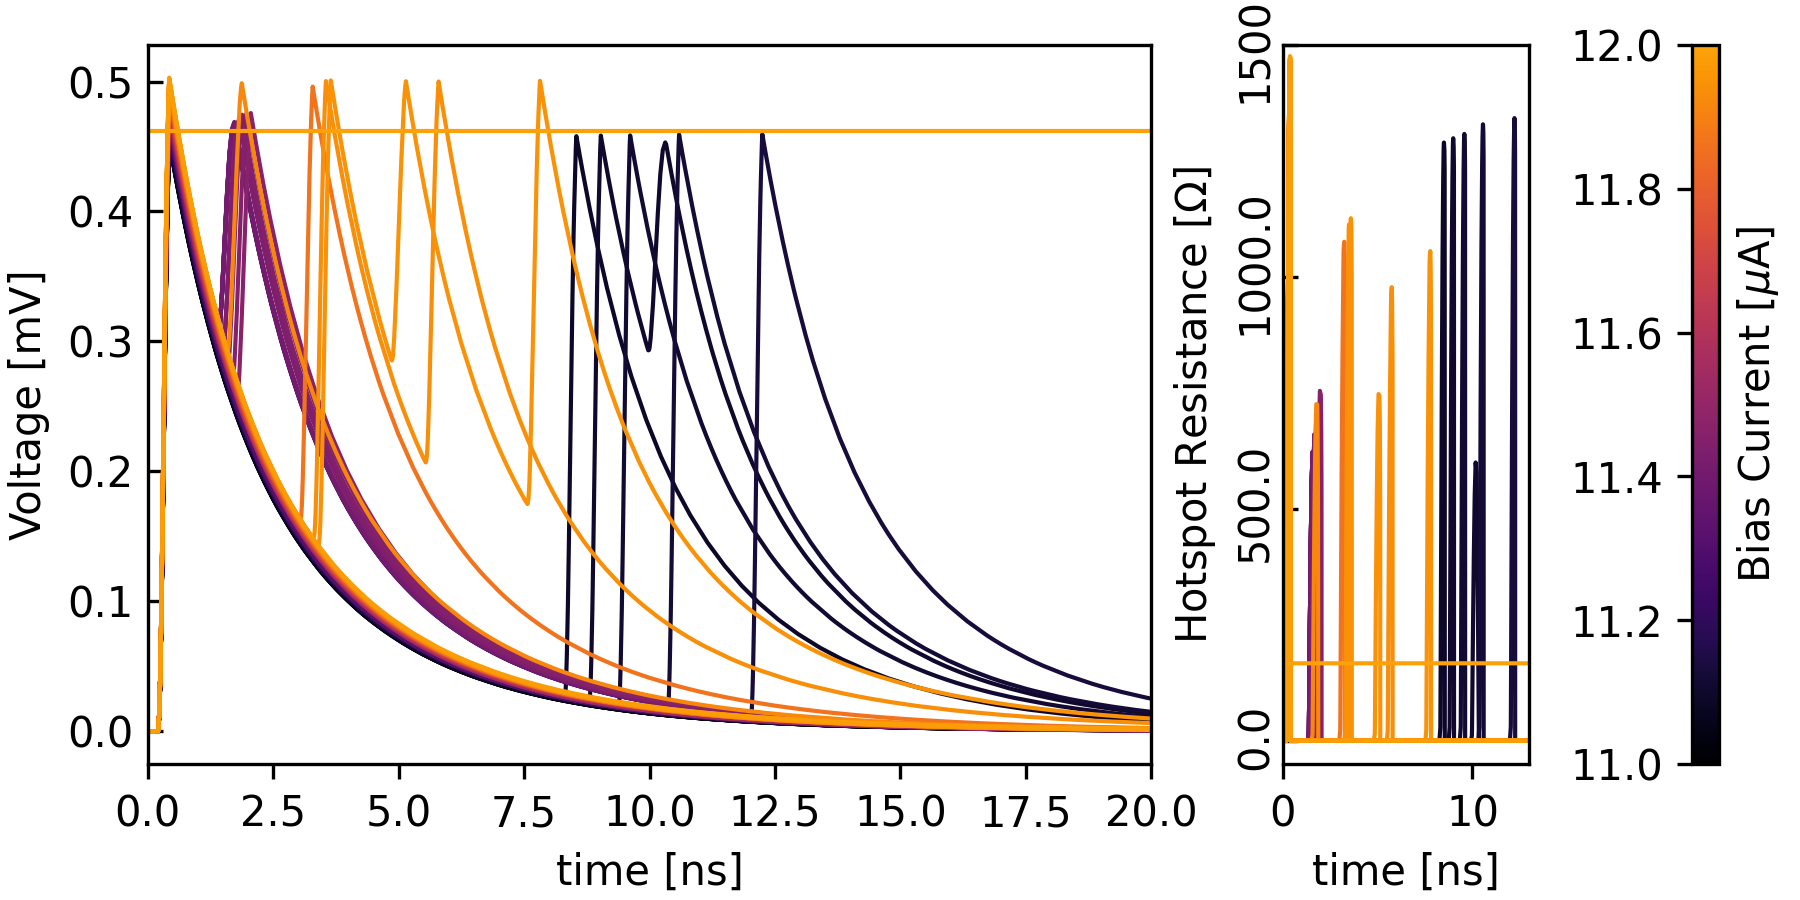
\includegraphics[width=0.8\textwidth]{figs/jumbled_mess_new.png}
    % }
    \caption{SNSPD readout circuit tested against 100 different bias values between
    $11\mu$A and $12\mu$A for a device with switching current $12\mu$A. The simulation
    was carried out using the existing nanowire model and the default options for LTspice
    on Mac (\cf{reltol} of $10^{-3}$, \cf{voltol} of $10^{-6}$, \cf{trtol} of $2$). 
    We expect to see only
    one pulse at $10$ns for all biases (except $12\mu$A). The instability of the model is
    related to the ratio of correct and incorrect simulations.}
    \label{fig:sweepbias}
\end{figure}

% these references are not as good, but may be worth checking out?
% https://gist.github.com/turingbirds/c90672c3b126d0d5f37f90494d5057cb
% https://www.eevblog.com/forum/projects/lt-spice-convergence/

Relative tolerance in SPICE is a simulation parameter that imposes a convergence criterion.
It is typically imposed in the form \cite{accurate_sim_in_spice_kundert}:
$$|v_{k+1} - v_k| \leq \cf{reltol} \cdot \max(|v_{k+1}|, |v_k|) + \cf{vntol}$$

This imposes a condition on the change in node voltage $v$ between iterations $k$ and $k+1$.
\cf{vntol} is equivalent to the voltage resolution and should be at least one order of magnitude
smaller than any node voltage (including the thermal integrator, more on that in section
\ref{current_nw}. Even though the nanowire might be a 2-port element (ignoring the photon port),
the relative tolerance is a check performed on the entire circuit. This implies that the relative
tolerance needs to satisfy this constraint on all logic inside the nanowire.

\subsection{Behavioral Sources}

Dependent sources are a powerful model in SPICE software that allows their output to be
dependent on other node voltages and currents. Along with the multiple types
of dependent sources that are supported by SPICE (e-, f-, g- and h-sources), LTspice
supports an additional type of dependent source called the behavioral source (b-source).
Behavioral sources can mimic the behavior of any other source type and additionally
can have multiple inputs (as opposed to the other sources' dependence on only one value).
B-sources also allow for the use of arbitrary math functions that allow them to compute
non-trivial expressions, such as time integrals, derivatives and modulos.
B-sources can use the outputs of functions defined using the \cf{.func} directive
as a current, voltage, resistance and power outputs (resistance and power aren't well 
documented). 

\begin{figure}
    \centering
    \subfigure[]{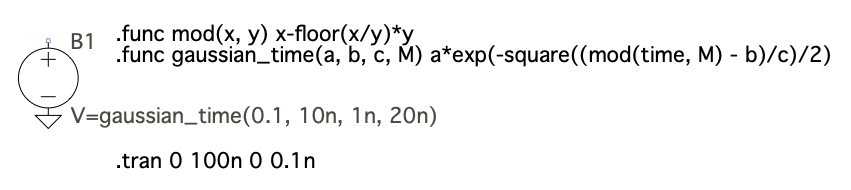
\includegraphics[width=0.8\textwidth]{figs/gaussian_src_circuit.png}
    \label{fig:gaussian_src_circ}}
    \subfigure[]{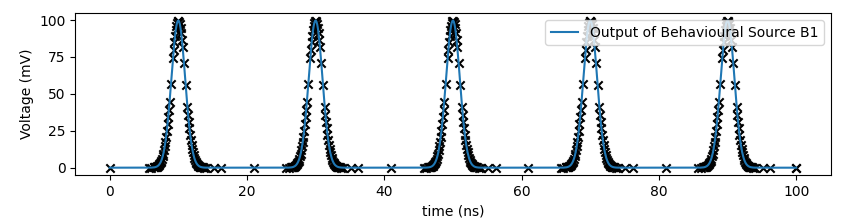
\includegraphics[width=0.8\textwidth]{figs/gaussian_src_output.png}
    \label{fig:gaussian_src_out}}
    \caption{Example of a behavioral source outputting gaussian pulses.}
\end{figure}

For example, one can construct a gaussian pulse source using dependent sources
by defining the two functions \cf{mod} and \cf{gaussian\_time} as shown in 
\ref{fig:gaussian_src_circ}.
% \begin{lstlisting}[language=python]
% .func mod(x, y) x-floor(x/y)*y
% .func gaussian_time(a, b, c, M) a*exp(-square((mod(time, M)-b)/c)/2)
% \end{lstlisting}
Using a b-source expression \cf{V=gaussian\_time(0.1, 10n, 1n, 20n)}
outputs a gaussian pulse with magnitude $0.1V$ with peaks
spaced out by $10$ns with a standard deviation of $1$ns as shown in figure
\ref{fig:gaussian_src_out}. 

B-sources are a helpful tool when designing circuits for stability as they
allow you to abstract complexity away from the circuit topology and remove 
reliance on \cf{reltol}. They can also function as state variables and perform
math on expressions that have varying output values -- such as performing math
on outputs that differ by more than 6 orders of magnitude. 

\section{Malicious Circuits} \label{malicious_circuits}

One method proposed to test for the stability of a nanowire model is by enumerating
the number of false switching events. In the same fashion that the state nonlinearity
can be used to amplify single events of small magnitude, the model can be used to 
nanowire count erroneous state crossings. If a simulation $\Sigma_C$
of a nanowire circuit $C$ accesses a state $\Sigma_C( u(t=0), T ) = u(T)$ after
a time $T$ using a finite method,
then running the same method with more steps should yield $u(T)$ if the method
converges \cite{DAHLQUIST}.
However, if the projections taken between simulation steps due to criterion 
based convergence introduce some deviation $\varepsilon$ at time $t'$ from the 
true circuit state, then the final solution will evolve from an $\varepsilon$ lightcone
away from $u_C(t')$. In a linear system, the $\varepsilon$ lightcone might be hard to
distinguish as $\Sigma_C(u(t=0), T) + \Sigma_C(\varepsilon, T-t') \approx \Sigma_C(u(t=0), T)$. 

However, since the nanowire's state is non-linear, if the $\varepsilon$ deviation happens
near a switching event, then the projection has a probability of switching the 
nanowire. By enumerating simulations of a nanowire varying the timestepping,
we can force the find the frequency of $\varepsilon$ errors occuring from switching
events.

Unfortunately, we can't perform this enumeration by varying timesteps in LTspice 
trivially. One workaround however, is simulating a circuit $C'=C+M$ that contains
the original circuit $C$ and a new malicious circuit $M$. $M$ does not have to be coupled
to $C$ topologically (a particularly simple and interesting case is when $M$ and $C$ are topologically
decoupled: sharing no nodes, 
currents or behavioral coupling).
$C$ and $M$ however are always time coupled: if $M$ exhibits a strong non-linearity
and smaller timestepping to account for that, then the simulation of $C$ also experiences 
finer timesteps. This time coupling allows
for enumerating simulations of $C$ without manually modifying the timesteps taken.

One example malicious circuit $M$ could be a voltage source exhibiting a pulse 
with a magnitude at least as big as $(\cf{voltol})/(\cf{reltol})$\todo[]{verify this ratio}
as shown in figure \ref{fig:w_malicious_circ_diag}.
This forces the simulator to use finer steps near the pulse edges and as a result
introduces some timestep variation to $C$ as well. Another example malicious circuit 
could be a one-way coupled circuit, such as a behavioral source with an output coupled
to a node in $C$ and amplifies its magnitude. This is equivalent to having the simulation
tolerances be different for one node in the circuit.

A special case for $M$ is the transmission line. The inclusion of a transmission line
in SPICE creates breakpoints that force the timestepping resolution for the entire simulation
to be below half the total line delay \cite{hspice, spice-book}. One possible enumeration would
be varying the delay of an \cf{LTRA} (O- or T-models). This works even when the transmission line
is not connected to anything.

\begin{figure}
    \centering
    \subfigure[]{
    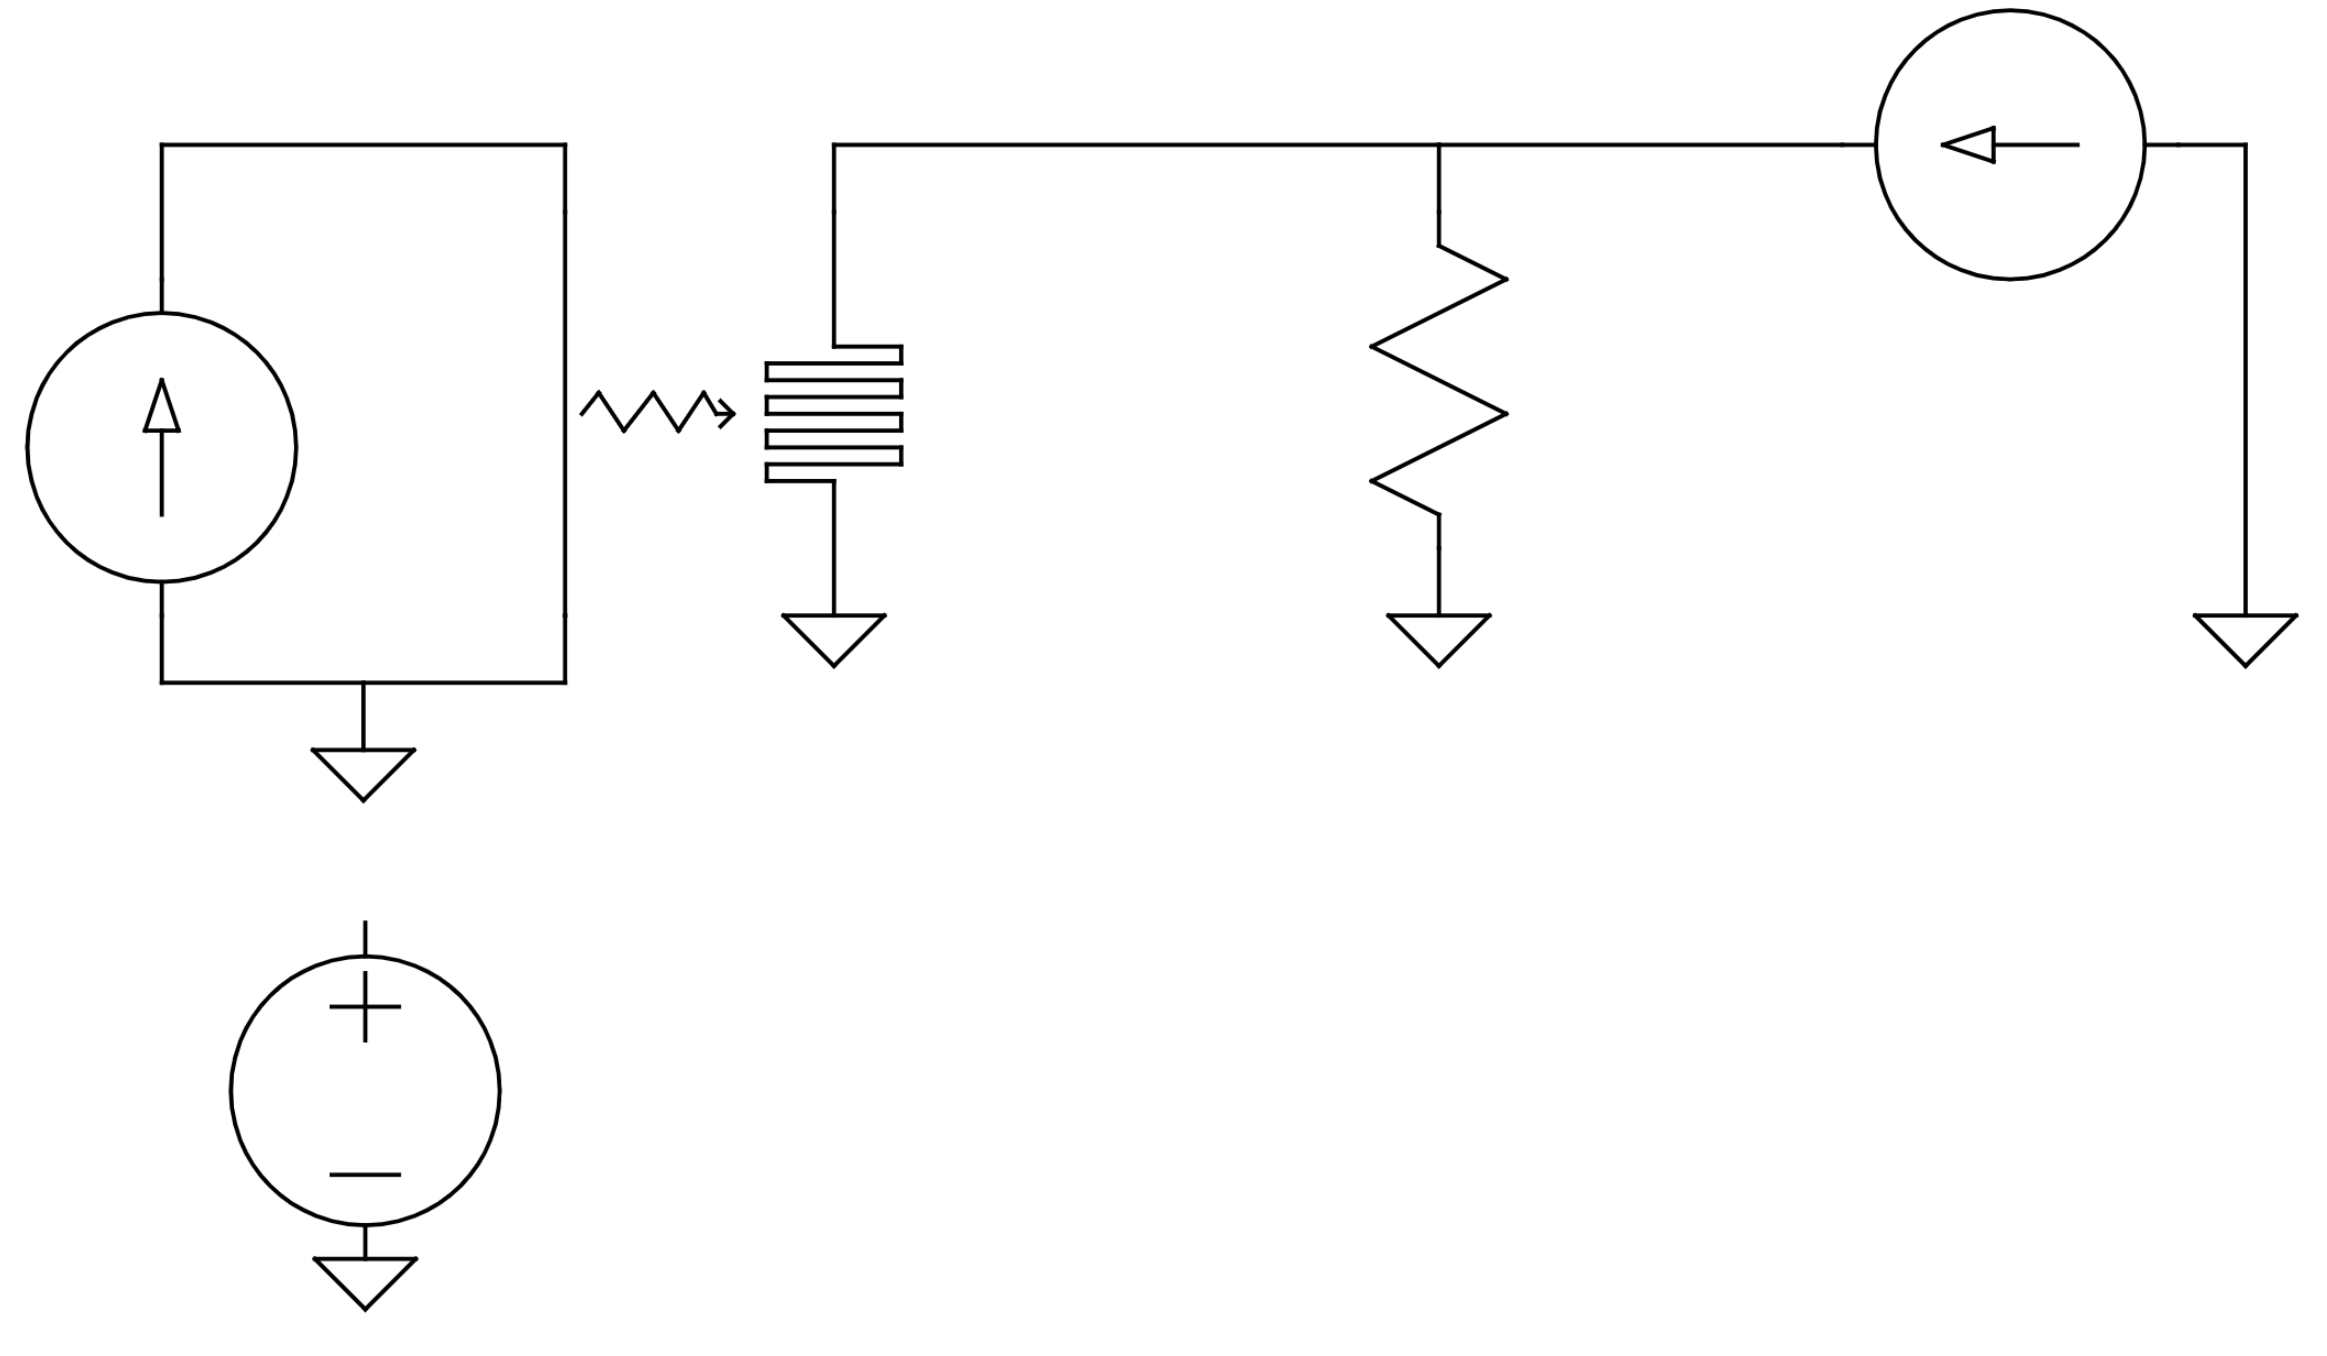
\includegraphics[width=0.4\textwidth]{figs/w_malicious_circ_diag.png}
    \label{fig:w_malicious_circ_diag}
    }
    \subfigure[]{
    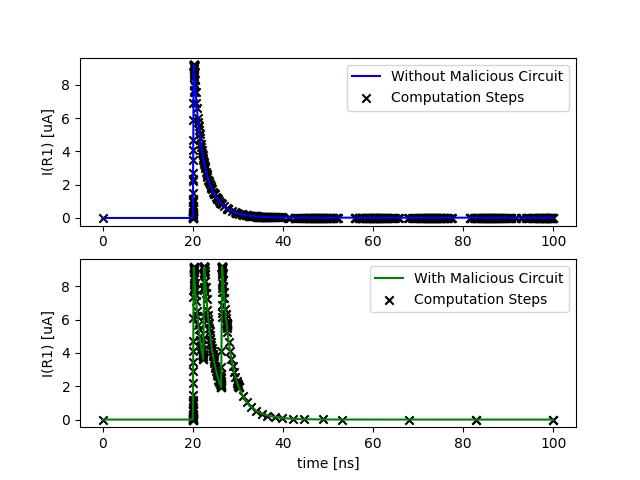
\includegraphics[width=0.55\textwidth]{figs/w_malicious_circ.png}
    \label{fig:w_malicious_circ}
    }
    \caption{(a) diagram of the circuit tested with a bias current of $11.1\mu$A and a photon incident at $20$ns on the existing nanowire model. The bottom circuit is a ``malicious circuit,'' it is a pulse source that produces a $10$ns square pulse during the evolution of the hotspot. (b) The top plot showcases a single hotspot forming when simulating
    the SNSPD circuit without the malicious circuit included. The bottom plot shows the evolution when the malicious circuit
    is included. The bottom plot shows multiple oscillations with peaks even though it should only show one. The
    malicious circuit projected errors on the hotspot evolution and caused the nanowire model to switch when it wasn't supposed to. The crosses indicate the individual timesteps the solver computed the waveform at.}
\end{figure}

Figure \ref{fig:w_malicious_circ_diag} shows a typical SNSPD readout circuit biased with $11.1\mu$A
and a decoupled
malicious voltage source. By running a simulation with and without that malicious subcircuit,
we can see that the inclusion of a malicious circuit affects the output result in figure
\ref{fig:w_malicious_circ}. Note that the resulting solution is not possible given the
typical geometry, even though it looks plausible, since the period of oscillations is not 
regular. Since we know the malicious voltage source in no way affects the main circuit,
we know that our model is unstable over time steps taken by PULSE sources. Note that
not all bias currents misbehave, but by sweeping a range of bias values, we are able to
find a couple that don't work as shown in figure \ref{fig:sweepbias}. About $6\%$ of
bias values output inconsistent results for a sweep with between $11\mu$A and $12\mu$A 
in steps of $10$nA.

This method can be extended to detect the stability of linear systems by coupling
a non-linear discriminator $D$ to the circuit $C$ and testing the stability by simulating
$C+D+M$. The discriminator $D$ needs amplify $\varepsilon$ deviations, the most straight-forward
way of doing that projects a node value from $C$ onto a finite field. For instance $D$ 
could be a behavioral source with an expression similar to $V=\cf{IF}(\cf{n001}>10\mathrm{u}, 1, 0)$ 
to couple to node \cf{n001} in circuit $C$. $D$ should have no effect on the operation of $C$,
any operation change in $C$ is an indicator of instability of $C$.

\todooptional[]{fig: malicious circuit examples}

% \subsubsection{Proof of Equivalence to Stability}

\section{Improving the Nanowire Model}

Now that we have a method to measure the stability of a subcircuit, we can use that
to measure and improve the nanowire model. The nanowire model's constituent subcircuits are
tested separately using the Malicious Circuits method to assign a relative stability
score. Using that method, we can highlight what subcircuits of the nanowire model are unstable 
and change the topology such that their governing dynamics are the same as the old subcircuit
but don't impose the same instability over the timestepping algorithm.

\subsection{Current nanowire model}
\label{current_nw}

Berggren et al.'s nanowire model comprises of four sub-circuits outlined in figure \ref{fig:old_nw}. The main subcircuit (subcircuit a), consists of a
non-linear inductor in series with a b-source in parallel with a resistor.
The non-linear inductor simulates the continuously non-linearity due to kinetic inductance,
while the resistor and b-source simulate switching and hotspot dynamics.
Subcircuit (b) stores the value of the boolean state tracking 
whether the nanowire is in the normal or superconducting state.
Subcircuit (c) is the hotspot integrator, the subcircuit is the
circuit analog for the hotspot integral solving for the node voltage $v_3$
which represents the hotspot resistance. Subcircuit (d) is an input port for
photons.

\begin{figure}
    \centering
    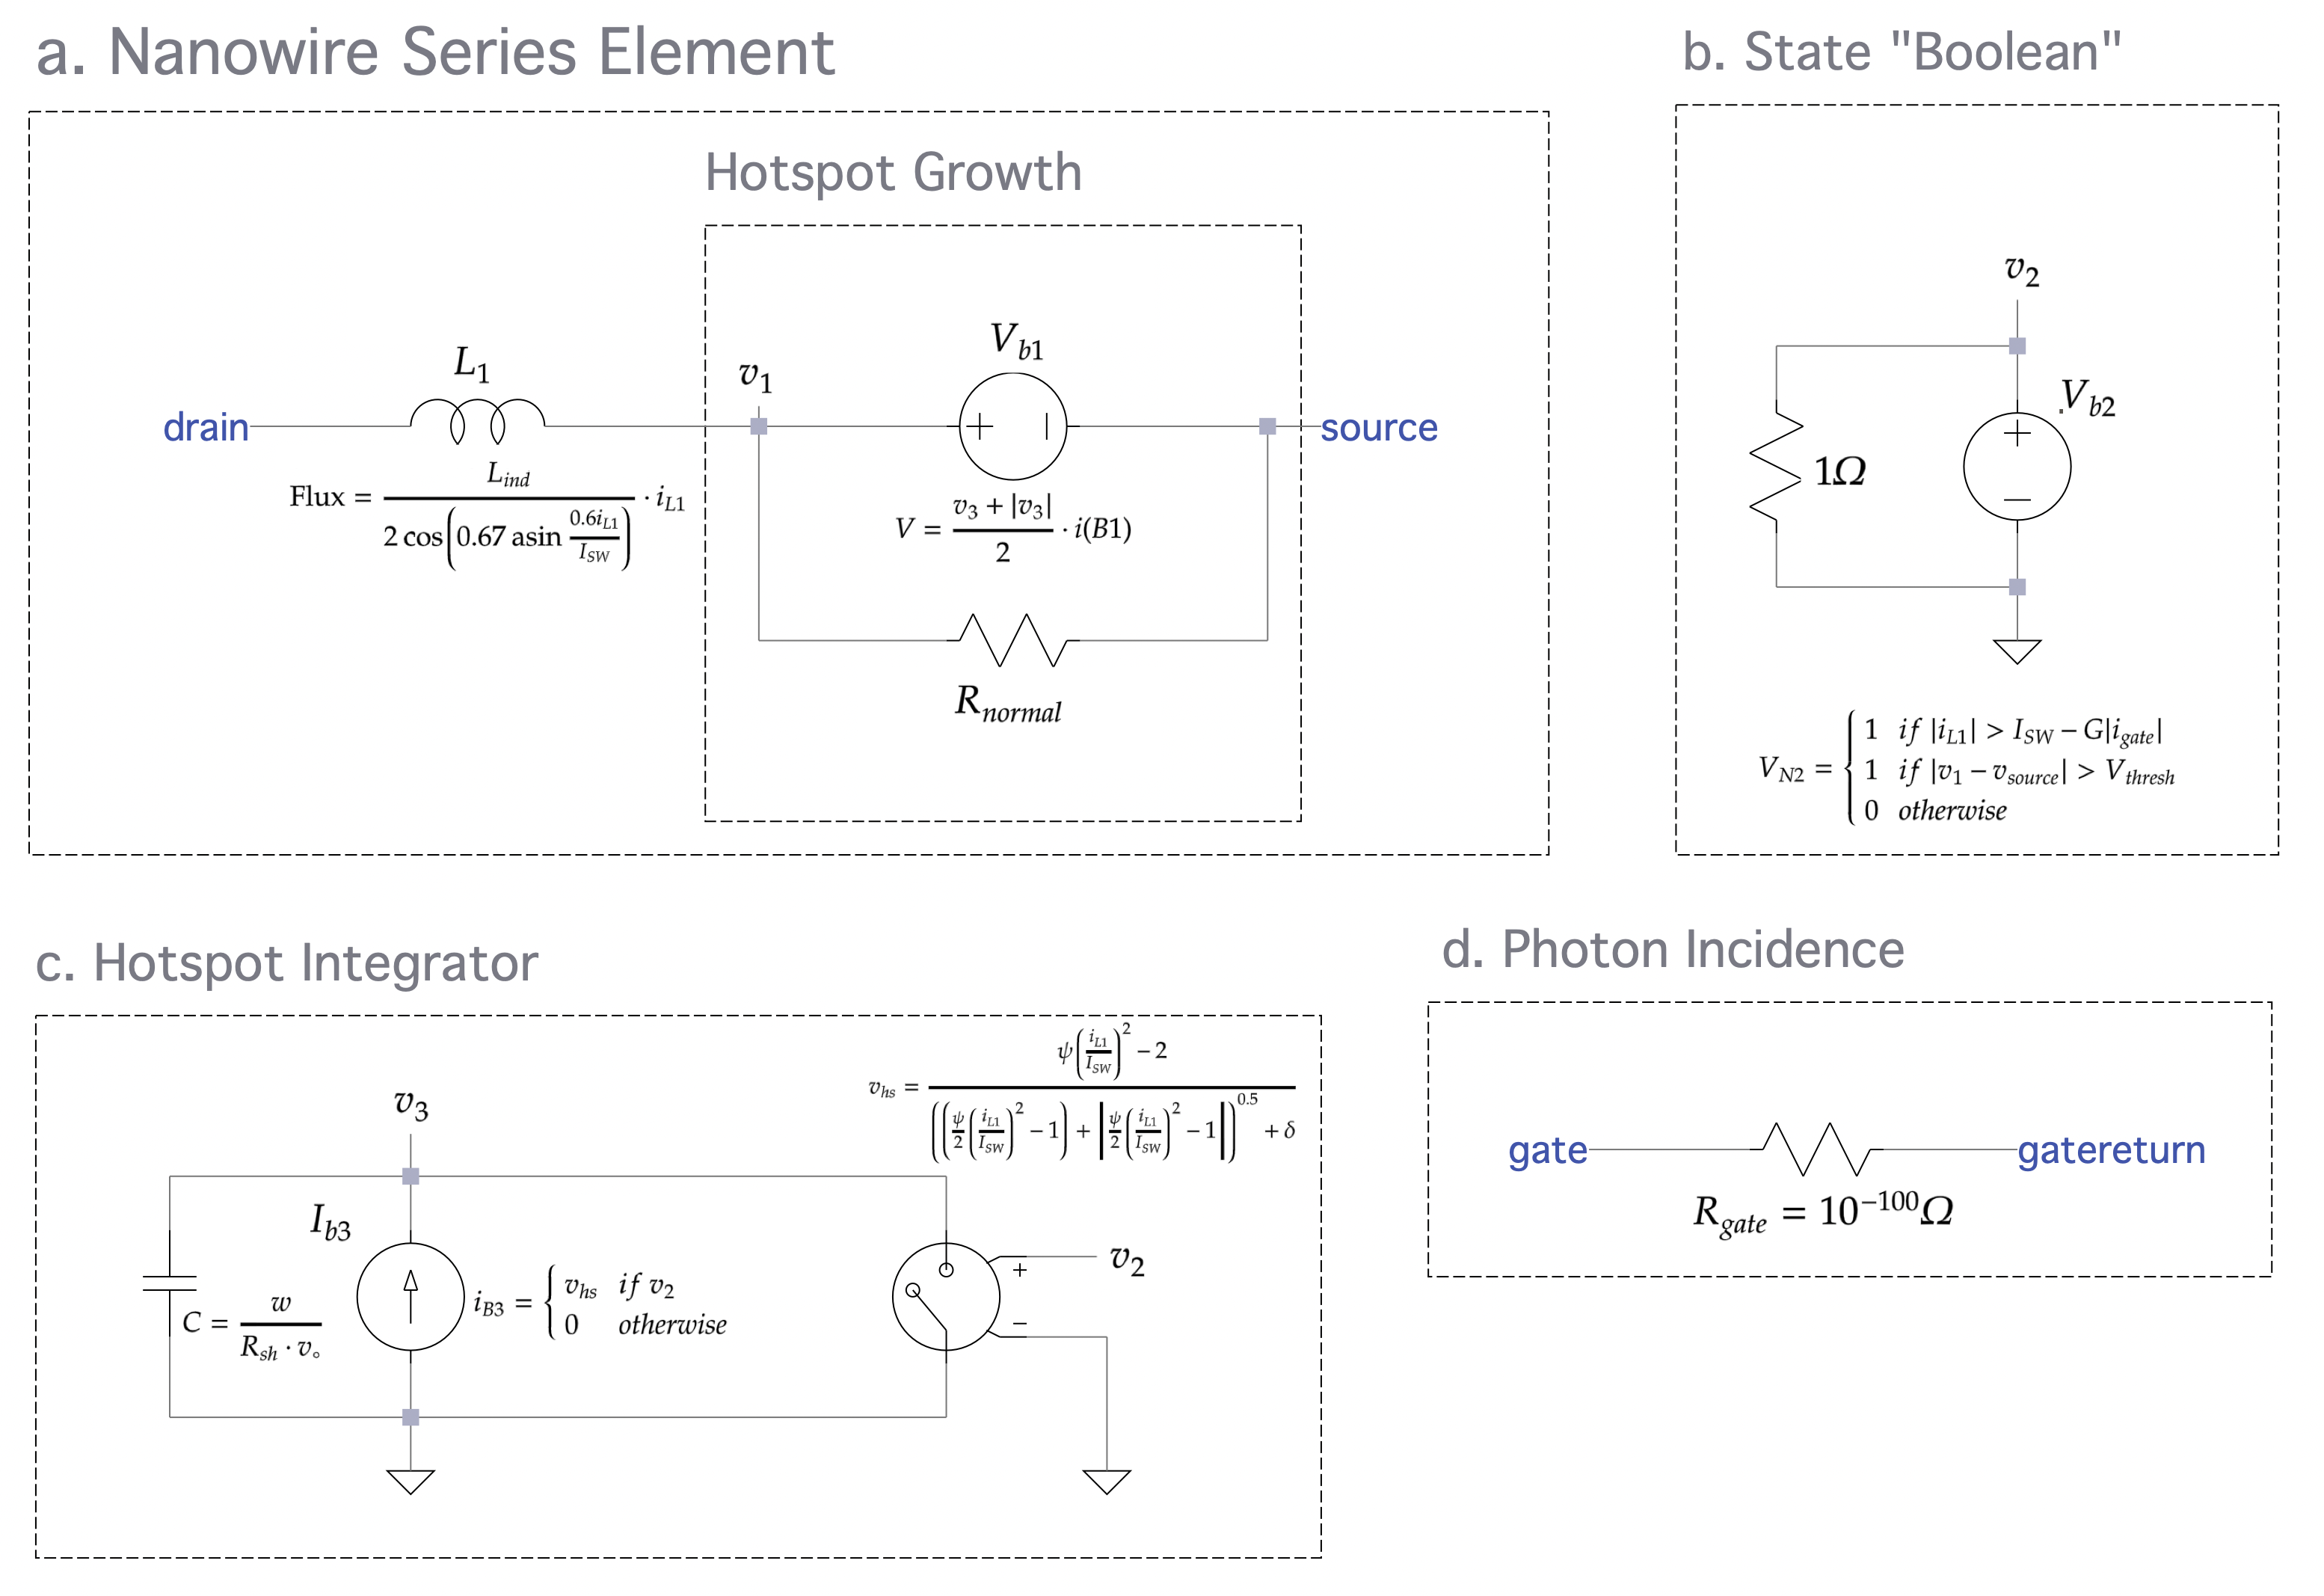
\includegraphics[width=\textwidth]{figs/old_nw.png}
    \caption{Diagram showcasing the four subcircuits used in the 
    Berggren et al. SPICE dynamic nanowire model. 
    Subcircuit a accounts for the kinetic inductance
    continuous non-linearity and the resistance in the normal state. Subcircuit b
    tracks a boolean state of superconducting vs. normal. Subcircuit c integrates
    the hotspot velocity as per the phenomenological hotspot model. Subcircuit
    d is the photon inlet.
    \todofig[inline]{remove the Rgate text from this fig}}
    \label{fig:old_nw}
\end{figure}

\begin{figure}
    \centering
    \begin{tikzpicture}[scale=1,auto=center,every node/.style={circle}]
      \tikzset{vertex/.style = {shape=circle,draw,minimum size=4em,fill=white}}
        \tikzset{edge/.style = {->,> = latex'}}
        \def\size{8em}
        % vertices
        \node[vertex] (b1) at  (360/7 * 0:\size) {$V_{b1}$};
        \node[vertex] (n1) at  (360/7 * 1:\size) {$v_1$};
        \node[vertex] (n2) at  (360/7 * 2:\size) {$v_2$};
        \node[vertex] (n3) at  (360/7 * 3:\size) {$v_3$};
        \node[vertex] (r3) at (360/7 * 4:\size) {$i_{gate}$};
        \node[vertex] (s1) at (360/7 * 5:\size) {\small{switch}};
        \node[vertex] (l1) at (360/7 * 6:\size) {$L_1$};
        %edges
        \draw[edge] [loop right] (b1) to (b1);
        \draw[edge] (b1) to (n1);
        \draw[edge] (n1) to (n2);
        \draw[edge] (n2) to (n3);
        \draw[edge] (n2) to (s1);
        \draw[edge] (n3) to (b1);
        \draw[edge] (r3) to (n2);
        \draw[edge] (s1) to (n3);
        \draw[edge] (l1) to (n2);
        \draw[edge]  (l1) to (n3);
    \end{tikzpicture}
    \caption{A dependency graph for some elements and nodes of the nanowire model as presented in
    figure \ref{fig:old_nw}. Each node in the graph represents
    a circuit node value that is calculated or an element parameter.
    Since the compiler is a black box,
    some degree and outdegree $1$ nodes were removed. Note that the time dependence
    of parameters is also removed, i.e. an edge to a variable could represent
    dependence in the same timestep or on the previous timestep of the value.
    This is a heuristic of how simulation parameters
    are dependent on each other, i.e. how stiffness or errors in one graph node couple to other nodes.}
    \label{fig:dependency_graph}
\end{figure}

Using dependency graphs, we can visualize how the model elements
are correlated in figure \ref{fig:dependency_graph}. 
By using directed graphs to represent execution 
order for nodes and element values, we can visualize the dependece
of parameters on each other. A system is said to have a dependency graph $G = (V, E)$
where $V$ represents variables as nodes and $E$ are the dependency edges.
A set of variables $V_1, V_2 \subseteq V$ are said to be decoupled if all nodes
in $V_1$ have node edges pointing to $V_2$ and vice versa. The dependency
graph for a system highlights how projection errors integrate over time.
\todoexplain[]{Explain why cycle, why thermal integrator projections...}
\todoref[]{citation from book Software Testing and Analysis: Process, Principles, and Techniques. Chapter 6}
\todoref[]{dragon book??}
%http://www.cs.toronto.edu/~chechik/courses16/csc410/dataflowReadings.pdf

The current nanowire model also currently lacks a DC part (operational mode) 
of the model.
LTspice DC solver struggles to efficiently represent a nanowire that is
undergoing relaxation oscillations (the solver tends to find that it is
switched) and misrepresents DC solutions for the superconducting state
as the normal state. This implies that for nanowire simulations,
the initial state of everything must be zero since transient analysis relies
on operational point analysis beforehand. Namely, all bias sources,
DC or not, should start at $0$. So a DC bias would be a \cf{PULSE} starting
at 0, ramping to a value and let it rest there for a bit. This is a by-product 
of LTspice not recognizing meta-stable systems. This is tackled by the new 
simulator introduced in section \ref{julia-sim-chapter}.

\subsection{Stability of the original nanowire model}

By varying the relative tolerance and testing different geometries, the value $10^{-6}$
seems to perform the best in terms of stability and accuracy. By testing the LC tank
geometry shown in \ref{fig:tank_circ} using a nanowire and swapping it with a linear 
inductor, we can test several \cf{reltol} values and see if we see the expected 
oscillation behavior. Intuitively, as the relative tolerance value used gets smaller,
the circuit should be ``more correct'' than when allowing for a bigger tolerance.
For the nanowire model, we don't see that behavior. Relative tolerances between $10^{-3}$
and $10^{-7}$
consistently worked in our tests, producing a sinusoidal oscillation. Values
above $10^{-7}$ either switch into the resistive state and lose all the energy immideatly
or oscillate in a decaying fashion. Meanwhile, for the SNSPD readout configuration,
we see consistently better behavior using the malicious circuits method presented in
\ref{malicious_circuits} as we go from $10^{-3}$ to $10^{-6}$ across photon events
and relaxation oscillations.

Even with a \cf{reltol} value of $10^{-6}$, the existing nanowire model is highly unstable
and can be improved through stability analysis.
Using Malicious Circuits, we test multiple operation regimes for
the nanowire and study the stability of every sub-circuit separately. Namely,
we care about the nanowire behavior in 4 different regimes: 
(1) as an inductor and resistor when normal, 
(2) as an inductor when superconducting, (3) the hotspot evolution when a photon is
incident, and (4) relaxation oscillation regime. We test these different regimes 
using one circuit with one nanowire element across \cf{reltol} values of $10^{-3}$
and $10^{-6}$ and compare it to the expected solution.

\subsection{Different Integrator}

The malicious circuits analysis on the old model indicated
that the integrator circuit is the main source of instability. 
We replaced it with a behavioral source that integrates the same hotspot
and observed an improvement in overall behavior.
This model is mathematically identical to the previous one with 2 changes
to the implementation: (1) use a built-in integrator instead of the circuit
integrator (subcircuit c) and (2) replacing $\frac{x+|x|}{2}$ with a conditional
on $x>0$ (or bound $x$ by the \cf{limit}).

The LTspice built-in integrator is better handled
by spice than the integrator's circuit equivalent model.
It involves doing one operation instead of increasing the circuit
matrix size. 
This approach not only involves creating fewer projections onto the circuit 
(leading to fewer errors)
but using the built-in integrator allows LTspice to better keep track of integration
time and shorting to ground. Note that the new integrator using the built-in
\cf{sdt} math command uses a reset condition. This condition is better handled as it
doesn't involve decreasing the timestep in a projective fashion as with circuit
non-linearities. The reset condition is substituting the switch that shorts $v_3$
to ground in figure \ref{fig:old_nw}. When the $v_2=0$ (wire is superconducting),
the integrator resets to the initial condition $0$.

The previous nanowire model also involved the switch toggling between the off and on
state with resistances of \qty{1}{m\Omega} and \qty{10}{G\Omega}. This switching behavior
introduces a strong non-linearity that can be better handled by the reset method
used by the \cf{sdt} command. In SPICE, a resistance changing value by an order of
$10^6$ instantly is unstable, let alone a magnitude of $10^{15}$. This magnitude
change coupled with using a lower \cf{reltol} leads to a large instability that
should be avoided.

Replacing $\frac{1}{2}\left(x+|x|\right)$ with an IF statement (or limit) allows the circuit matrix compiler to
have an easier time optimizing the simulation. The evaluation of this statement results in $x$ if $x>0$, otherwise
$0$.
While $\frac{1}{2}\left(x+|x|\right)$ preserves continuity,
a carefully crafted \cf{IF} statement can exhibit the same continuity. 
In this case, the function we are trying to replicate with an \cf{IF} statement is not
continuous, it would be harder to perform this optimization, however, since continuity is
preserved, the speedup offered is not at the expense of stability.
This implies that no advantage from a
convergence standpoint is offered, however, the compiler has to perform multiple operations instead of
evaluating one conditional. The limit math command is a built-in way of handling this as well, where the
lower limit is $0$ and the upper limit is the peak hotspot resistance. While the implementation of the limit
command is unknown, its implementation (and accompanying optimization) should intuitively be similar to that
of an IF statement. These two methods also allow for greater readability than the absolute value conditional.

\begin{figure}
    \centering
    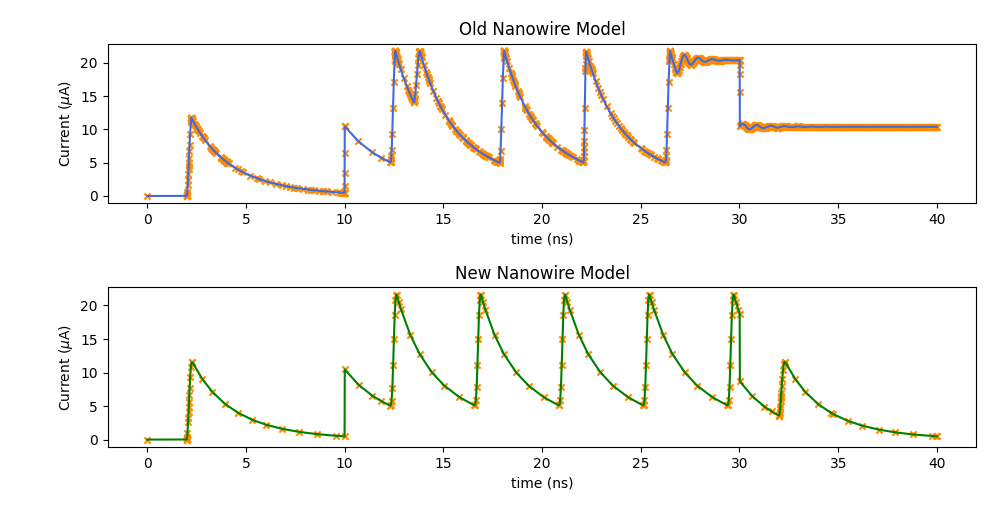
\includegraphics[width=0.9\textwidth]{figs/int_improvement_1e-3.png}
    \caption{Comparison of the old and new nanowire model that replaces the
    circuit integrator with the internal LTspice resetting integrator. Solid
    lines represent the output waveform and the crosses are the values evaluated at each
    individual timestep. Photons are incident at $2$ and $32$ns on a wire biased by $15\mu$A.
    The bias is increased to $25\mu$A between $10$ and $30$ns to enter the wire into the
    relaxation oscillation regime.We see that in this example, the new model is more accurate, as well as, requiring fewer discrete timesteps to solve the equation at.}
    \label{fig:int_improvement_1e-3}
\end{figure}

\begin{figure}
    \centering
    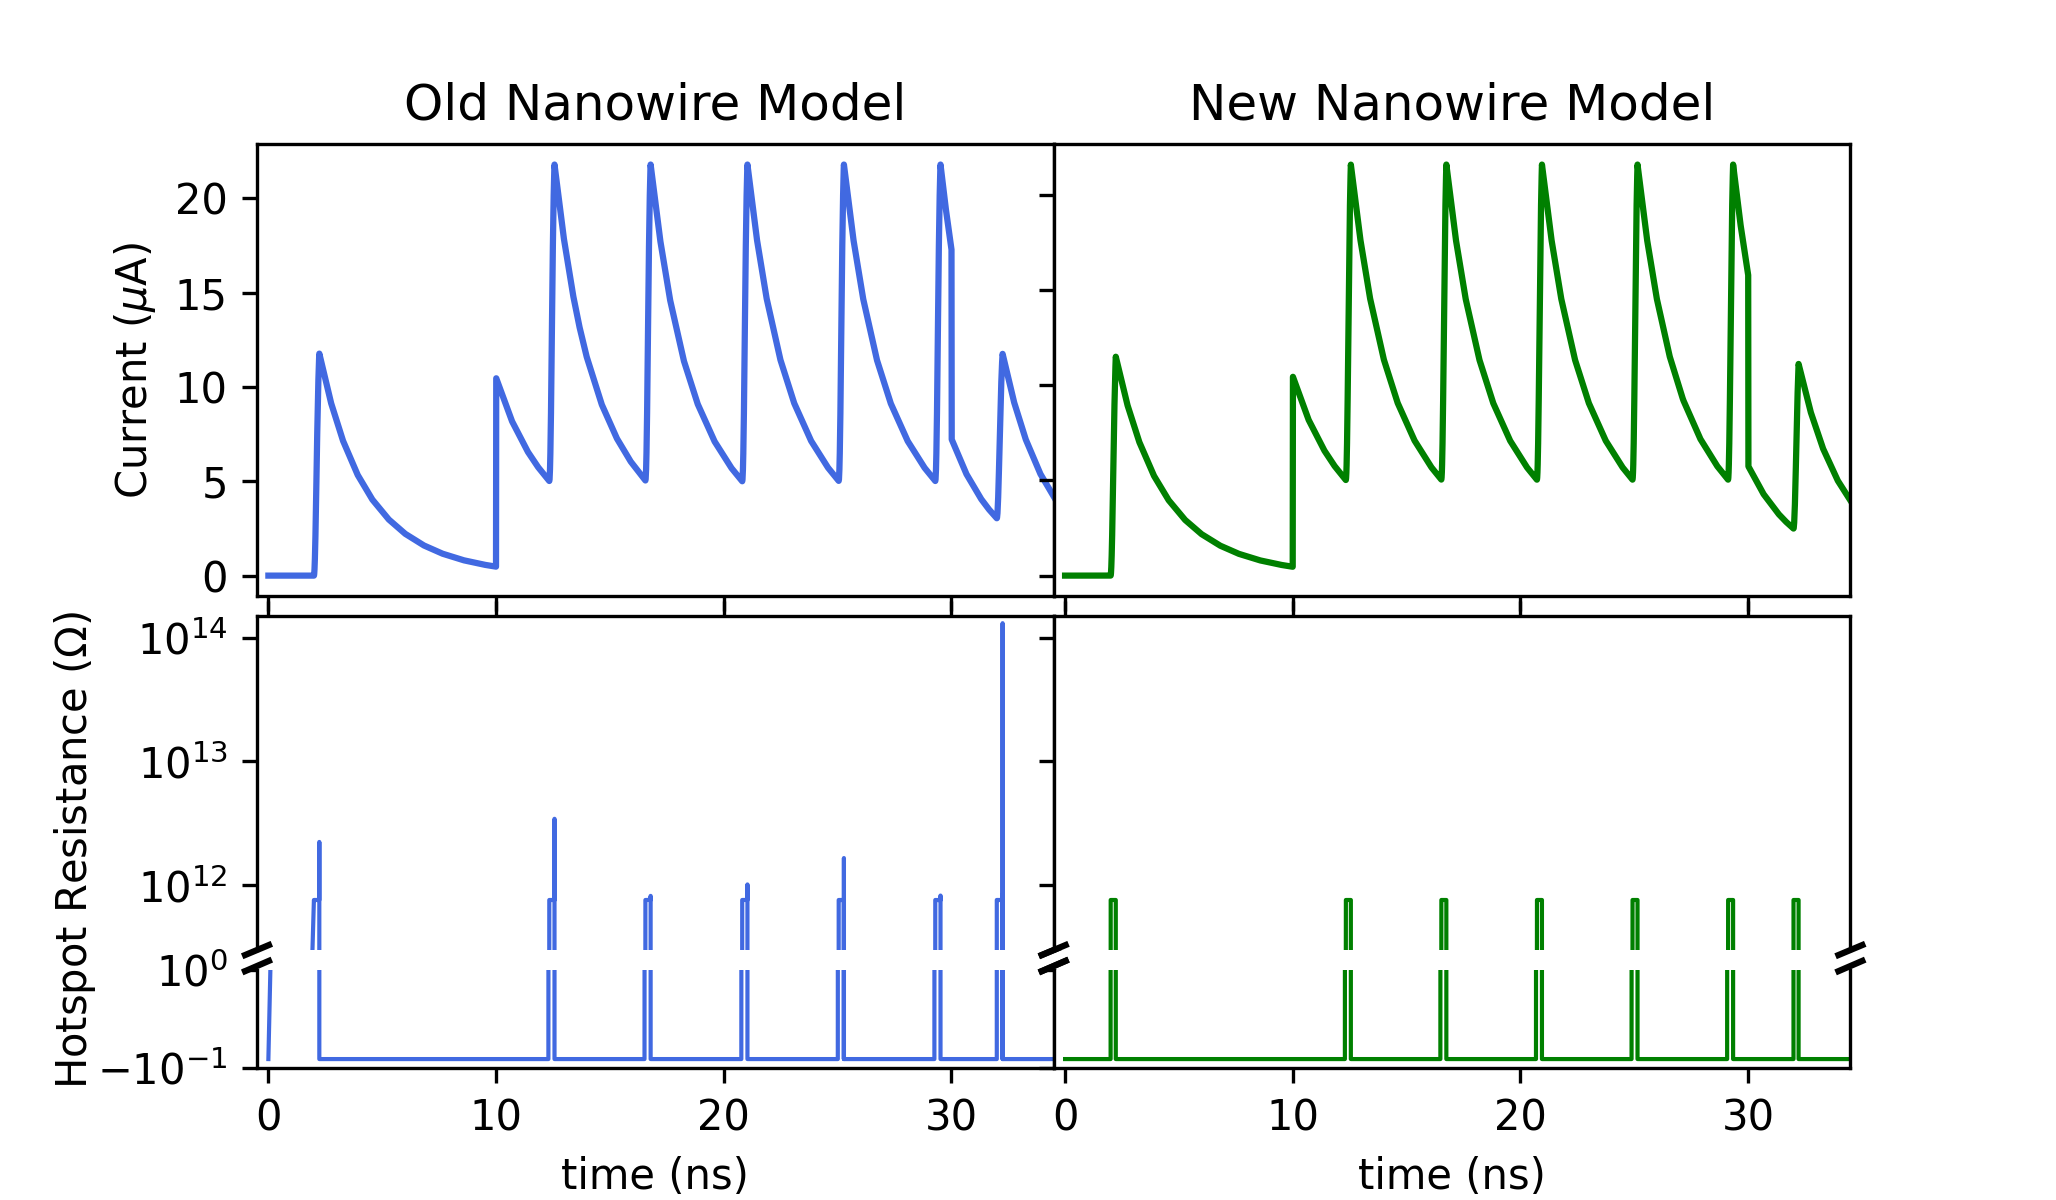
\includegraphics[width=0.9\textwidth]{figs/int_improvement_1e-6.png}
    \caption{For the same setup in figure \ref{fig:int_improvement_1e-3}, we see
    that both models seem to perform well on readout when using a \cf{reltol} value
    of $10^{-6}$. However, the hotspot resistance is unstable in the old model peaking
    up to $2$ orders of magnitude above the actual value.}
    \label{fig:int_improvement_1e-6}
\end{figure}

Along with more accurate simulations of the behavior of the nanowire, we also
observe the simulator using fewer time steps overall (fewer crosses in figure 
\ref{fig:int_improvement_1e-3}). This corresponds to faster convergence and also is
an indicator of fewer projections that needed to be done, indicating less
error over the binary state. Needing fewer points to solve a system suggests
linearity. In this case, we can observe that the model can comfortably relax
back into linearity when the pulse magnitude is constant and there is no
switching behavior occurring. The higher density of datapoints in the improved model 
is reserved for the beginning of the state non-linearity transition (hotspot growth region)
as opposed to being employed during the entire evolution in the old model.

Figure \ref{fig:int_improvement_1e-6} compares the performance of the old and new 
nanowire models at a \cf{reltol$=10^{-6}$}. This example is for the same bias as in 
figure \ref{fig:int_improvement_1e-3}, where the current output seems correct.
However, looking at the hotspot resistance by scoping the internal variables of the 
model, we see that the hotspot resistance has huge spikes, up to 2 orders of magnitude
above the correct value. This is a source of instability in the model that can also
be analyzed using Malicious Circuits, even though the hotspot resistance itself is
a combined measurable ($R_{\mathrm{hotspot}} = \frac{v_1 - v_{\mathrm{source}}}{i}$).

\begin{figure}
    \centering
    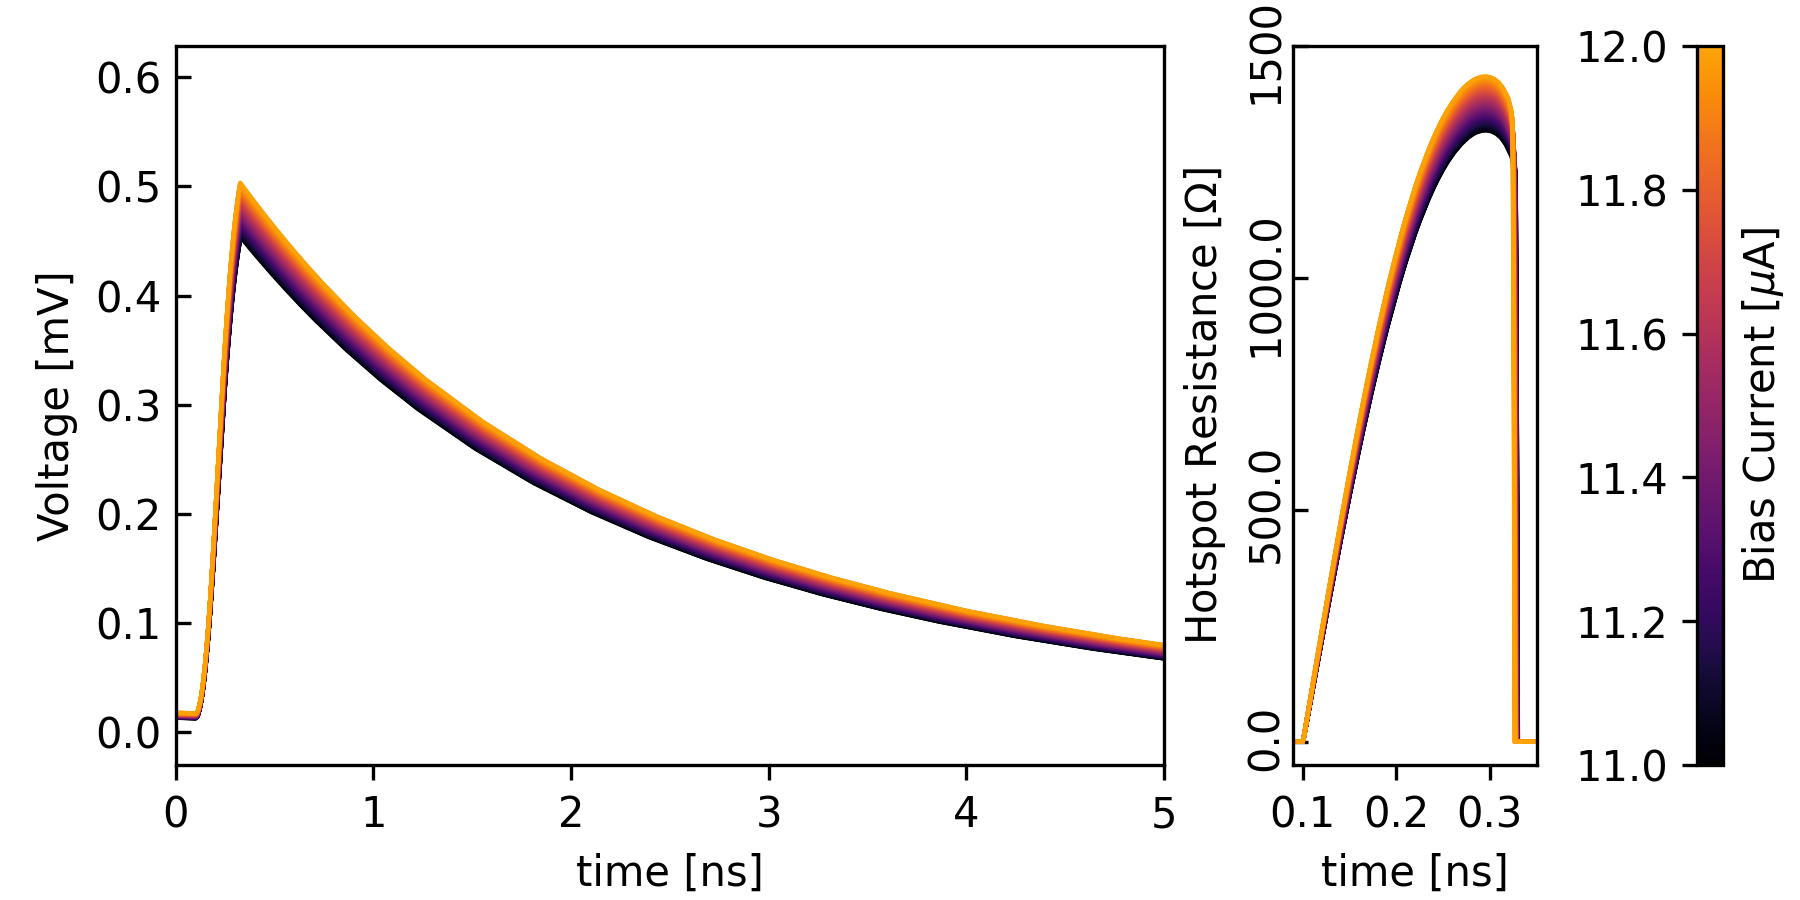
\includegraphics[width=0.8\textwidth]{figs/not_jumbled_mess.png}
    \caption{A sweep of bias currents on the new nanowire model with a photon detection event.
    $100$ equally spaced bias values between $11\mu$A and $12\mu$A were tested. We observe
    a smooth gradient of the resultant
    hotspot resistance and voltage spike that is much more consistent than the old nanowire
    as shown in figure \ref{fig:sweepbias}. 
    }
    \label{fig:not_jumbled_mess}
\end{figure}

We can see the same sweep performed on the original nanowire in figure \ref{fig:sweepbias}
performed on the model with improved stability in figure \ref{fig:not_jumbled_mess}. We can see
a smooth gradient of responses form as the bias increases (as opposed to random activity seen
in the old model). This is expected, as the device should experience one harsh state non-linearity.
After that transition, the system to should be continuously non-linear in a fashion that can be simulated
by transient simulations accurately. We also can see the hotspot peak resistance increase smoothly
with the bias current in the new model, while witnessing the hotspot decaying faster. This showcases
that our model is directing current to the shunt at a faster rate -- allowing the wire to cool back into the
superconducting state earlier on.

\subsection{1-Element Models}

Collapsing a sub-circuit to one element can provide speed and convergence advantages, especially for
nonlinear elements, at the risk of instability past a certain point. This method can be useful in
applications where the nanowire is used in one configuration repeatedly. For example, in the SNSPI
model generated in section \ref{snspi_dyn_model}, replacing the nanowire element with a behavioral
one-element model that spikes the resistance upon a photon incidence without integrating the entire
hotspot velocity. This can be done by precomputing the effect of the bias in a program like spice-daemon
and reusing that computed value or by loading multidimensional PWL tables into LTspice.

A good resource for one-element models are behavioral sources (b-sources). B-sources can operate
in the voltage (BV source) and current source (BI source) mode with their outputs set by an arbitrary 
maths expression
which can be a function of global parameters such as node values. B-sources can also behave
as behavioral resistors (BR) and power sources (BP), these two modes aren't well documented.
BR sources are useful candidates for modelling hotspots, as they can have a 0 resistance that spikes
to the hotspot peak resistance. The tolerances are more lenient for a BR than a BV source across
a resistor. The nanowire model has a small $10^{-3}\omega$ resistance, which is inconsequential for
most simulations. Care should be taken when using a BR source starting at zero resistance as it
may cause convergence issues if nonlinear effects trigger smaller timesteps near the switching
threshold.

Precomputing switching behavior outside LTspice can be done by modelling any complicated thermal
model in outside software and imported into LTspice via \cf{spice-daemon}. This could involve stripping
nanowires from the hotspot integrator and having voltage spikes output across it as a normal
nanowire would have given the bias the resistor is experiencing. Since \cf{spice-daemon} can access
simulation data, the nanowire bias can be deduced either explicitly from the YAML file or by
running an initial DC simulation to determine the nanowire bias.

Multidimensional tables can also be computed for nanowires and imported into LTspice. While
LTspice does not
support 2D tables or interpolation, it only supports 1D piece-wise-linear (PWL) interpolation
through the built-in \cf{table(x, x1, y1, $\cdots$)} command \cite{ltspice-bsource-wiki}. However
this 1D interpolation function can be used as a well-convergent 2D interpolator by discritizing
the search space using a finite number of squares (which is remappable to 1D), then implementing
the 2D interpolation using built-in LTspice math commands. For example, a 
2D map on $x, y$ evaluating to $f(x, y)$ can be encoded 
by enumerating each square with the diagonal points $(x, y)$ and $(x+\Delta x, y + \Delta y)$ and 
computing $f$ at the corners of each square. This
enumeration is linear, one general example mapping is $M(x, y) = \frac{1}{k_x}\floor{k_xx}+G\cdot \frac{1}{k_y}\floor{k_yy}$ where
$k_x, k_y$ are related to the resolution ($\Delta x, \Delta y$) and $G$ is related to $\max{x}$
and $k_x$. 
The mapping $M(x, y)$ evaluates to one unique number for each pair $x, y$ on the corners
of the squares. We can now interpolate any function $f$ across that range for any two query points 
$x', y'$ by evaluating
a function $f$ over the points $M(x, y), M(x+\Delta x, y), M(x, y+\Delta y), M(x+\Delta x, y+\Delta y)$.
The weighted sum of these evaluations is a 2D linear interpolation. A different simpler method could be
used (such as rounding) for a 2D table with no interpolation. The basic principle for encoding higher 
order maps into LTspice is to convert
the space to a finite enumerated map, compute the target function over the corners of each square and
encode that using the \cf{table} math command. 

These models require less operations and checks per iteration, allowing for faster compute. 
These models are ideal for large scale simulation, such as simulating thousands of nanowires.
Using
a behavioral source with finitely many operations takes less than 6 operations per iteration and
acts on one node. Even in a sparse setting, arbitrary subcircuits span multiple entries and force
a larger number of operations a second - many resulting from individual \cf{reltol} (and other tolerance)
checks. Using a macro-model to encode the behavior of the nanowire decreases the number of possible
stability issues. However, these macro-models encode a finite number of interactions, and as such, can 
act in a behavior that seems correct (since it is hard coded) when it is not. This motivates being
extra careful with models designed for high performance and large-scale system modeling. Having an
environment controlled check to validate the sensibility of a circuit output is a useful add-on. For
example, having the pre-compute workflow in \cf{spice-daemon} compute the behvioral model and the
post-compute workflow check that when the nanowire switched, the current in the device was above
the critical current, a photon was incident, etc. 

\section{Outlook and applications}

This chapter demonstrated a simple stability analysis technique for SPICE solvers that involves
counting malicious circuits --  uncoupled circuits that affect each others output through
timestep coupling. This method can be used to highlight unstable subcircuits or elements of a 
model to improve the model's stability. We use this to analyse the stability of the nanowire 
model to show that the hotspot integrator is highly unstable and is the main culprit for
erroneous switching events seen when using the nanowire model. By replacing the hotspot 
integrator with a behavioral source reset-equipped integrator, we showcase a much more stable
and accurate nanowire model. We also find that the most well-convergent relative tolerance 
for both nanowire models is $\cf{reltol}=10^{-6}$ and is essential when considering the
state nonlinearity.

The increase in the stability of the nanowire model is essential when scaling up devices: 
as the number of nonlinear models increases, erroneous switching events become more prevalent
and hard to distinguish from regular events. The more new more stable model also showcases a
speed improvement when being simulated. This method can be extended to work on both nonlinear
and linear circuits by coupling to a malicious circuit.